\section{Maple to Semantic \LaTeX{} Translator}\label{sec:backward-translation}
Instead of writing a custom \Maple{} syntax parser, we using \Maple's internal data structure to get a syntax tree of the input\footnote{In consequence, a license of \Maple{} is mandatory to perform backward translations. The translator is using the version \Maple{} 2016.}. \Maple{} allow different input styles. The \texttt{1D} input is mainly used for programming purposes and therefore also used to perform our translations. Internally, \Maple{} using \gls*{dag} as syntax trees.

\begin{wrapfigure}{r}{0.61\textwidth}
	\vspace{-22pt}
	\centering
	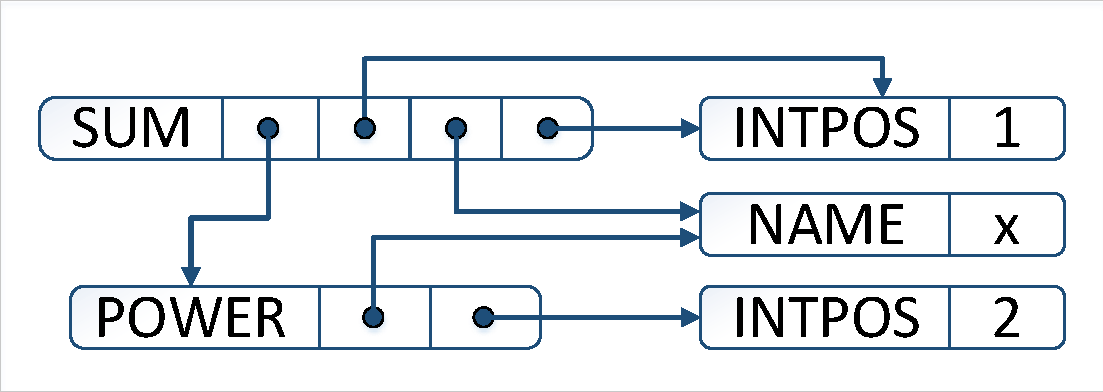
\includegraphics[clip, trim=0.5cm 0.5cm 0.5cm 0.5cm, scale=0.5]{DAGreal.pdf}
	\vspace{-5pt}
	\caption{The internal \Maple{} DAG representation of $x^2+x$.}
	\label{fig:internal-maple-dag}
	\vspace{-15pt}
\end{wrapfigure}

Each node in the \gls*{dag} stores its children and has a header, which defines the type and the length of the node. Consider the polynomial $x^2+x$. Figure~\ref{fig:internal-maple-dag} illustrates the internal \gls*{dag} representation with headers and arguments.

One can access the internal data structure of expressions via the \texttt{ToInert} command. The returned \inertF{} is a nested list representation as a tree equivalent\footnote{A tree equivalent of a \gls*{dag} splitting nodes with multiple parents into multiple nodes so that each node has only one parent node.} of the internal \gls*{dag} for the given expression. Some of the important types for the nodes are specified in \Cref{tab:maple-types}.

\begin{table}[h]
\centering
\begin{tabular}{cp{10cm}}
	\hline
	Type & Explanation\\
	\hline
	SUM & Sums. Internally stored with factors for each summand, i.e., '$x+y$' would be stored as '$x \cdot 1 + y \cdot 1$'.\\
	PROD & Products.\\
	EXPSEQ & Expression sequence is a kind of list. The arguments of functions are stored in such sequences.\\
	INTPOS & Positive integers.\\
	INTNEG & Negative integers.\\
	COMPLEX & Complex numbers with real and imaginary part.\\
	FLOAT & Float numbers are stored in the scientific notation with integer values for the exponent $n$ and the significand $m$ in $m \cdot 10^n$.\\
	RATIONAL & Rational numbers are fractions stored in integer values for the numerator and positive integers for the denominator.\\
	POWER & Exponentiation with expressions as base and exponent.\\
	FUNCTION & Function invocation with the name, arguments and attributes of the function.\\
	\hline
\end{tabular}
\caption{A subset of important internal \Maple{} data types. See~\parencite{MAPLE:ProgrammingGuide} for a complete list.}
\label{tab:maple-types}
\end{table}

%\subsection{Maple's Open Maple API}
The translator using the \texttt{OpenMaple}~\parencite[\S 14.3]{MAPLE:ProgrammingGuide} \gls*{api} for interacting with \Maple's kernel and get access to the \inertF{} of inputs.

\subsection{Automatic Changes of Inputs in Maple}\label{subsec:maple-probs}
\Maple{} evaluates inputs automatically and changes the input into an internal representation. This internal representation might look a bit different to the input. One example has already been given with \Cref{fig:internal-maple-dag}, where each summand of a sum is stored with a factor. Here is a list of all internal changes that occur for inputs.

\begin{itemize}
\item \Maple{} evaluates input expressions immediately.
\item There is no data type to represent square roots such as $\sqrt{x}$ (or $n$-th roots). Therefore, \Maple{} stores roots as an exponentiation with a fractional exponent. For example, $\sqrt{x}$ is stored as $x^{\frac{1}{2}}$.
\item There is no data type for subtractions, only for sums. Negative terms are changed to absolute values times '$-1$'. For example, $x-y$ is stored as $x + y \cdot (-1)$. 
\item Floating point numbers are stored in the scientific notation with a mantissa and an exponent in the base $10$. For example, $3.1$ is internally represented as $31 \cdot 10^{-1}$.
\item There is only a data type for rational numbers (fractions with integer numerator and positive denominator), but not for general fractions, such as $\frac{x+y}{z}$. This will be automatically changed to $(x+y)\cdot z^{-1}$.
\end{itemize}

There are unevaluation quotes implemented to avoid evaluations on input expression. Table~\ref{tab:unevaluation-quotes} gives an example how those unevaluation quotes work.

\begin{table}[ht]
\centering
\begin{tabular}{lcc}
\hline
& Without unevaluation quotes & With unevalation quotes\\
\hline
Input expression: & \texttt{sin(Pi)+2-1} & \texttt{'sin(Pi)+2-1'}\\
Stored expression: & 1 & \texttt{sin(Pi)+1}\\
\hline
\end{tabular}
\caption{Example of unevaluation quotes for \texttt{1D} \Maple{} input expressions.}
\label{tab:unevaluation-quotes}
\end{table}

Since we want to keep a translated expression similar to the input expression, we implemented some cosmetic rules for the backward translations that solve or reduce the effects from the list of changes above. 
\begin{itemize}
\item We use unevaluation quotes to suppress evaluations of the input.
\item We perform reordering of factors and summands so that negative factors appear in front of the summand. This gives us the opportunity to translate $x - y$ to $x - y$ instead of $x + y \cdot (-1)$.
\item We introduced the new internal data types \texttt{MYFLOAT} and \texttt{DIVIDE} to translate floats and fractions in more convenient notations.
\end{itemize}

The translation process then follows the same principle as for the forward translations. Since the syntax tree of \Maple{} is an expression tree, we do not need to implement special reordering or grouping algorithms to perform backward translations. Translations for functions are also realized via patterns and placeholders. Figure~\ref{fig:backward-trans} illustrates the backward translation process for the Jacobi polynomial example from \Cref{tab:JacobiP-usecase}.

\begin{figure}[t!]
	\centering
	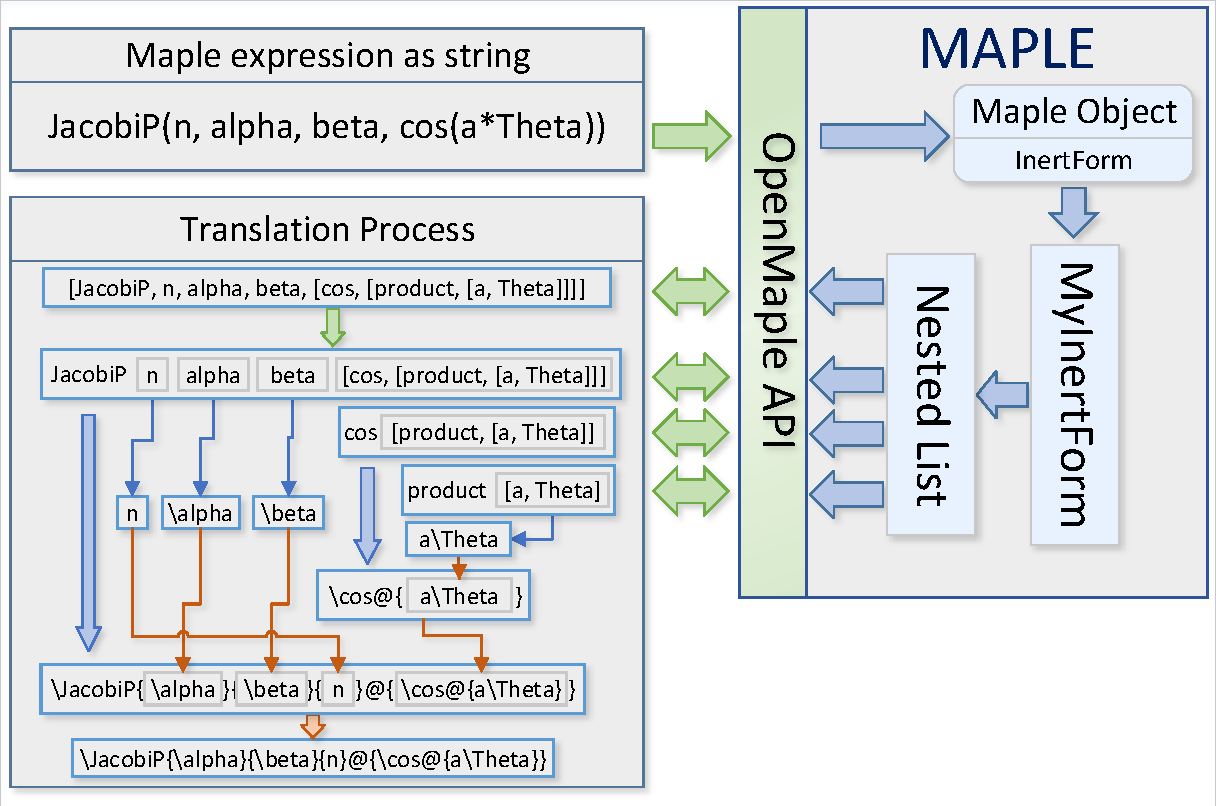
\includegraphics[clip, trim=0.1cm 0.1cm 0.1cm 0.1cm, scale=0.7]{MapleTranslation.pdf}
	\caption{A scheme of the backward translation process from \Maple{} for the Jacobi polynomial $P_n^{(\alpha , \beta)}(\cos(a\Theta))$. The input string is converted by the \Maple{} kernel into the nested list representation. This list is translated by subtranslators (blue and red arrows). A function translation (bold blue arrows) is again realized by translation patterns to define the position of the arguments (red arrows).}
	\label{fig:backward-trans}
\end{figure}
